% Generated by python -m scripts.render_report; do not hand edit.

\section{Trạng thái dữ liệu và phạm vi phép đo}

Corpus chính gồm 2.500 bài thuộc 10 lĩnh vực, 250 bài/lĩnh vực. Bộ 20 query có hai query/lĩnh vực. Pool dùng BiMM có 669 cặp, 0 nhãn confirmed; mẫu kiểm tra chéo gồm 134 cặp.

Ba baseline pooling: TF-IDF Cosine sublinear/smoothed/L2; binary presence Cosine không IDF; BM25 với $k_1=1{,}2$, $b=0{,}75$, IDF một lần. Cùng corpus và tokenizer, hợp Top-20; TF-IDF đã đối soát SearchEngine.

\textbf{P@10, Recall@10, F1@10, MAP và NDCG@10: chưa đo chính thức.} Nhãn pending không được biến thành relevance. Bảng theo query/lĩnh vực dưới đây là độ trễ thật, không thay cho chất lượng truy xuất.

\section{Môi trường và thiết lập}

Lần đo UTC: 2026-10-16T13:42:48.188882+00:00. Python 3.13.5; Windows-11-10.0.26300-SP0; CPU AMD64 Family 25 Model 117 Stepping 2, AuthenticAMD; 16 logical CPU.

Mỗi query lặp 100 lần, 5 lượt warm-up trên toàn query set, Top-10. Chỉ mục đã nạp; đo gồm chuẩn hóa, BiMM, lọc và truy xuất, không gồm khởi động Python/nạp từ điển/đĩa hay vẽ giao diện. C4 thuần và fallback C3 được đo độc lập.

\section{Kết quả độ trễ và dung lượng}

\begin{table}[htbp]
\centering
\begin{tabular}{|l|r|r|r|r|}
\hline
Cấu hình & Mean (ms) & P95 (ms) & Rỗng & Số đo \\
\hline
C1 & 0.994 & 1.992 & 0 & 2000 \\
C2 & 0.463 & 1.034 & 0 & 2000 \\
C3 & 0.772 & 1.737 & 0 & 2000 \\
C4 & 0.487 & 1.355 & 200 & 2000 \\
C4 + C3 & 0.503 & 1.226 & 0 & 2000 \\
\hline
\end{tabular}
\caption{Độ trễ trên corpus chính, BiMM thật.}
\end{table}

\begin{table}[htbp]
\centering
\begin{tabular}{|l|r|r|r|l|}
\hline
Cấu hình & Phục vụ (byte) & TDV (byte) & Giảm/C1 & Mục tiêu 30\% \\
\hline
C1 & 9621765 & 0 & 0.00\% & không đạt \\
C2 & 6987156 & 0 & 27.38\% & không đạt \\
C3 & 8748327 & 0 & 9.08\% & không đạt \\
C4 & 6542944 & 1834419 & 32.00\% & đạt \\
C4 + C3 & 15291271 & 1834419 & -58.92\% & không đạt \\
\hline
\end{tabular}
\caption{Dung lượng chỉ mục đơn và gói triển khai fallback.}
\end{table}

C4 thuần trả kết quả rỗng ở Q04, Q15; phép đo C4 + C3 dùng chỉ mục C3 riêng để khôi phục truy vấn, không giữ term đã bị xóa trong chỉ mục C4.

Mục tiêu mean dưới 30 ms: đạt. Tỷ lệ giảm âm có nghĩa dung lượng tăng. Phải giữ C3 nếu triển khai fallback; không sử dụng riêng dung lượng C4 để kết luận cho cả gói. Tốc độ thấp hơn không chứng minh relevance tốt hơn.

\begin{figure}[htbp]\centering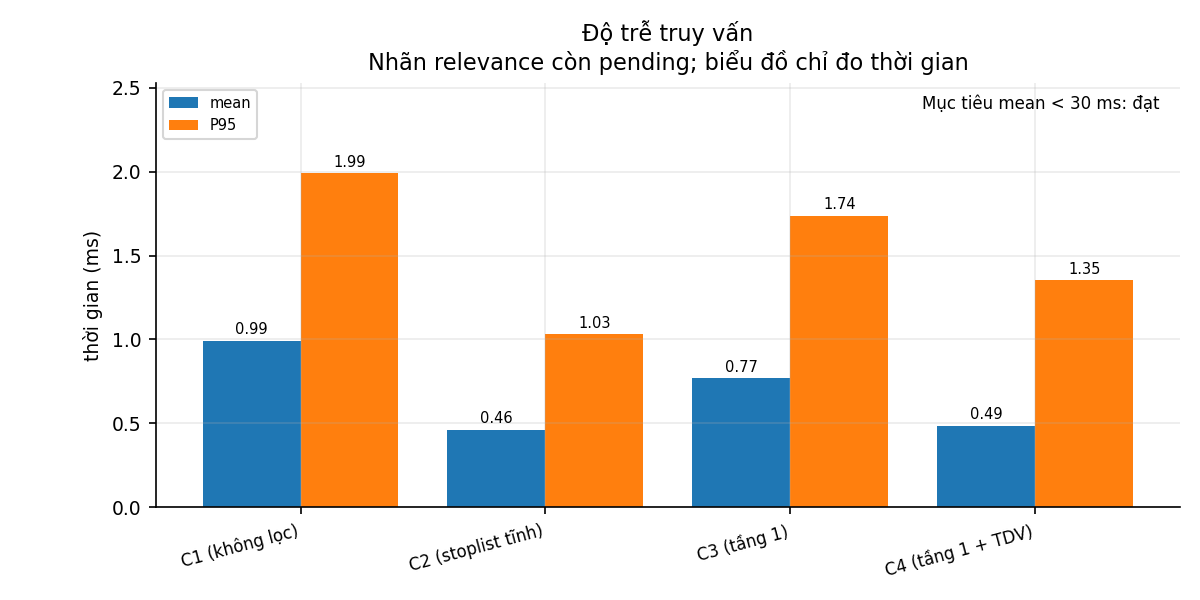
\includegraphics[width=.9\textwidth]{figures/fig_latency.png}\caption{Mean/P95 truy vấn BiMM.}\end{figure}

\begin{figure}[htbp]\centering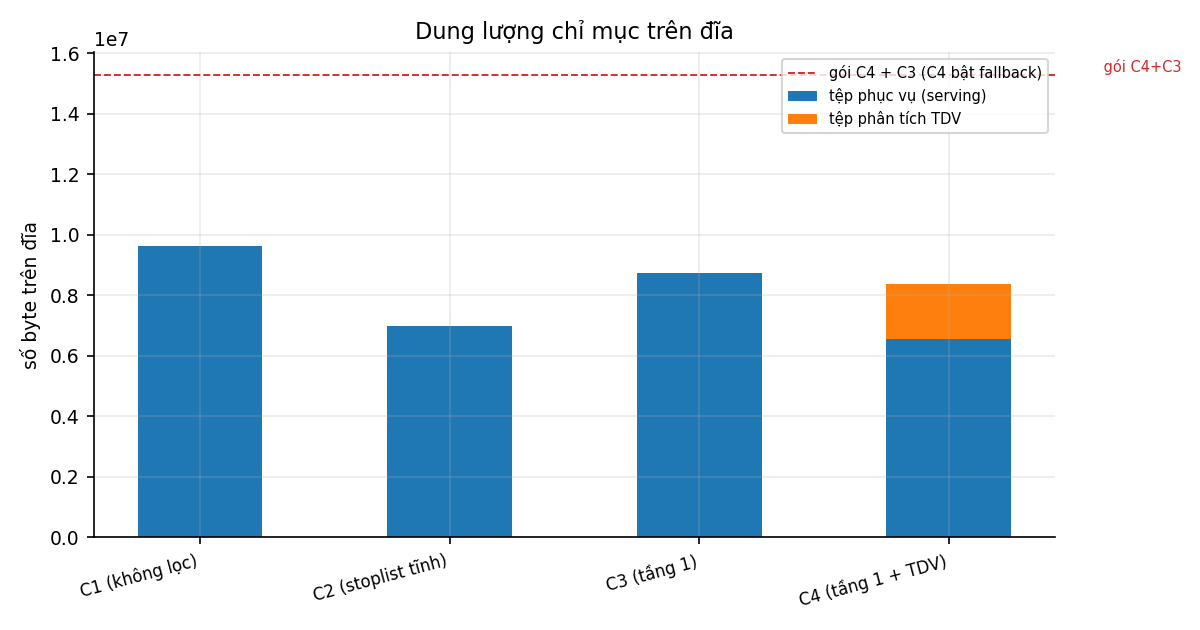
\includegraphics[width=.9\textwidth]{figures/fig_index_size.png}\caption{Dung lượng phục vụ, phân tích và gói fallback.}\end{figure}

\section{Thống kê TDV trên corpus đa lĩnh vực}

Mật độ gốc 0.03731830; chấm 31076 term, 666 điểm âm dưới dung sai. Bảo vệ 77 term theo whitelist/policy hợp từ; lọc thật 589 term. Thời gian TDV 12.641 giây, one-shot trên đủ 2.500 bài. Đây là tiêu chí hình học, không phải nhãn không liên quan ngữ nghĩa.

\begin{figure}[htbp]\centering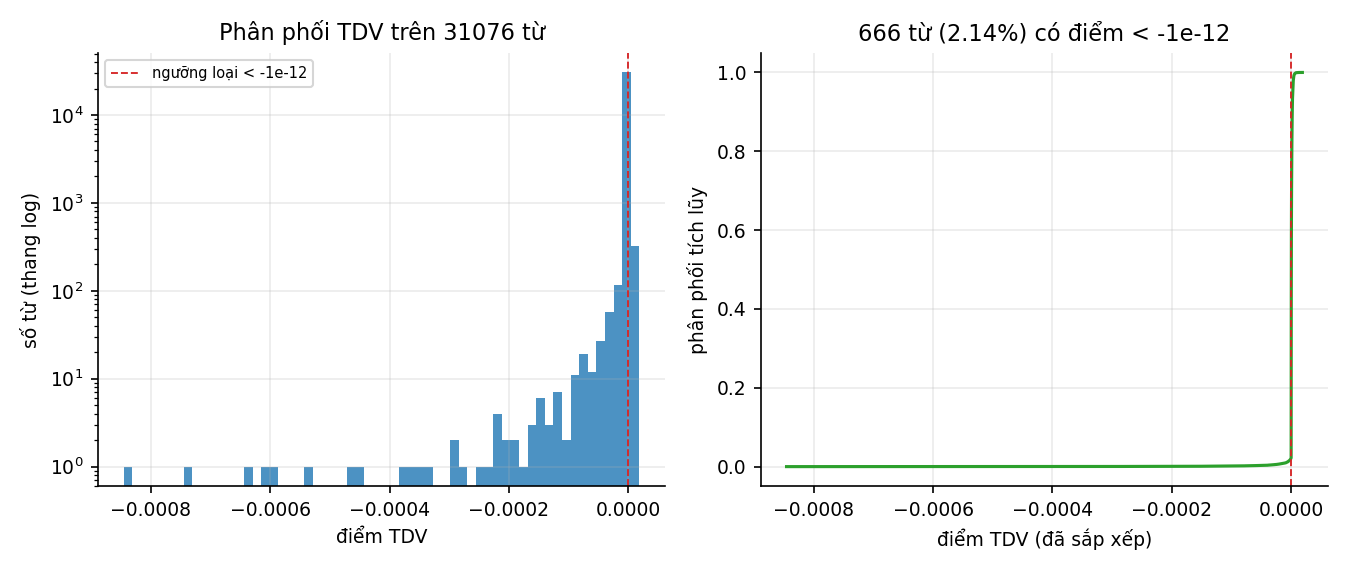
\includegraphics[width=.9\textwidth]{figures/fig_tdv_distribution.png}\caption{Phân bố TDV thực, không ép hình chữ U.}\end{figure}

\clearpage\section{Toàn bộ query và phân tích theo lĩnh vực}

\begin{longtable}{|l|p{.48\textwidth}|r|r|r|r|}
\hline
Query & Nội dung & C1 & C2 & C3 & C4 \\
\hline
\endhead
Q01 & lương tối thiểu & 0.153 & 0.091 & 0.188 & 0.089 \\
Q02 & biển cấm đỗ xe ô tô ở Hà Nội mất hiệu lực thì người dân đỗ xe ở đâu & 1.457 & 0.870 & 1.638 & 0.998 \\
Q03 & có nên tha thứ cho người vợ ngoại tình & 1.043 & 0.275 & 0.765 & 0.401 \\
Q04 & tâm sự gia đình & 0.198 & 0.244 & 0.162 & 0.031 \\
Q05 & nghiên cứu lõi băng để khám phá quy luật biến đổi khí hậu & 0.809 & 0.460 & 0.726 & 0.303 \\
Q06 & Trung Quốc xây trạm không gian và Nga phóng tàu lên ISS khác nhau như thế nào & 1.537 & 0.900 & 1.248 & 0.913 \\
Q07 & cổ phiếu & 0.066 & 0.055 & 0.107 & 0.079 \\
Q08 & lãi suất cơ bản và chính sách tiền tệ của Fed ảnh hưởng thị trường ra sao & 1.348 & 0.500 & 0.798 & 0.479 \\
Q09 & điều tra vụ biển thủ hơn 8,7 tỷ đồng cá độ bóng đá đã được xử lý ra sao & 1.596 & 0.502 & 1.377 & 0.379 \\
Q10 & đường dây chạy án trong vụ PMU18 & 0.833 & 0.289 & 0.362 & 0.238 \\
Q11 & ung thư & 0.064 & 0.087 & 0.074 & 0.102 \\
Q12 & mỡ máu cao nếu không điều trị có thể gây những biến chứng gì & 1.190 & 0.379 & 1.199 & 1.118 \\
Q13 & vì sao Mỹ vẫn chưa tìm thấy vũ khí cấm ở Iraq & 1.055 & 0.527 & 0.901 & 0.563 \\
Q14 & xác nhận danh tính hài cốt lính Mỹ mất tích trong Chiến tranh Triều Tiên & 1.037 & 0.697 & 0.653 & 0.457 \\
Q15 & vô địch & 0.091 & 0.117 & 0.144 & 0.019 \\
Q16 & Việt Nam đăng cai một vòng bảng Tiger Cup 2004 và các trận chung kết diễn ra thế nào & 1.723 & 0.814 & 1.499 & 1.388 \\
Q17 & cảnh nóng và trang phục hở trong phim truyền hình Việt Nam gây tranh luận như thế nào & 1.697 & 0.899 & 1.150 & 1.007 \\
Q18 & ca khúc và chương trình biểu diễn âm nhạc của nghệ sĩ & 1.182 & 0.464 & 0.502 & 0.275 \\
Q19 & virus máy tính đánh cắp mật khẩu Windows và cách phòng tránh & 1.224 & 0.412 & 0.643 & 0.351 \\
Q20 & dịch vụ phần mềm và thông tin di động được doanh nghiệp cung cấp cho khách hàng ra sao & 1.569 & 0.683 & 1.302 & 0.555 \\
\hline
\caption{Mean ms của toàn bộ 20 query.} \\
\end{longtable}

\begin{table}[htbp]
\centering
\begin{tabular}{|l|r|r|r|r|r|}
\hline
Lĩnh vực & Query & C1 & C2 & C3 & C4 \\
\hline
Chính trị – Xã hội & 2 & 0.805 & 0.481 & 0.913 & 0.543 \\
Đời sống & 2 & 0.621 & 0.259 & 0.464 & 0.216 \\
Khoa học & 2 & 1.173 & 0.680 & 0.987 & 0.608 \\
Kinh doanh & 2 & 0.707 & 0.277 & 0.452 & 0.279 \\
Pháp luật & 2 & 1.215 & 0.395 & 0.870 & 0.309 \\
Sức khỏe & 2 & 0.627 & 0.233 & 0.637 & 0.610 \\
Thế giới & 2 & 1.046 & 0.612 & 0.777 & 0.510 \\
Thể thao & 2 & 0.907 & 0.465 & 0.821 & 0.703 \\
Văn hóa & 2 & 1.440 & 0.681 & 0.826 & 0.641 \\
Vi tính & 2 & 1.397 & 0.548 & 0.973 & 0.453 \\
\hline
\end{tabular}
\caption{Mean ms theo 10 lĩnh vực; chỉ hai query/lĩnh vực.}
\end{table}

Mỗi lĩnh vực chỉ có hai query nên kết quả nhóm chưa đủ để suy rộng. Các bảng chất lượng toàn query/nhóm sẽ do evaluator xuất khi qrels đủ điều kiện, không thay dữ liệu thiếu bằng số 0.
